\documentclass{beamer}

\usetheme[]{Rochester}
\usecolortheme{beaver}
\usepackage[latin1]{inputenc}
\usepackage{graphics}

\author{Will Webberley}
\date{Autumn 2014}
\institute[COMSC]{Cardiff School of Computer Science and Informatics}



\title{Usability}
\subtitle{CM2101: Human-Computer Interaction}

\begin{document}

\frame{\titlepage}

\frame{
    \frametitle{Introduction to usability}
    Human-computer interaction is not just interface-building.
    \begin{columns}
        \column{.5\textwidth}
            \begin{block}{You need to be able to} 
                \begin{enumerate}
                    \item Understand system \alert{usability}
                    \item Design an \alert{efficient} UX
                    \item Engineer suitable \alert{task designs} and \alert{dialogues}
                    \item \alert{Evaluate} interface usability and performance
                    \item Use interface \alert{components} and \alert{design patterns}
                    \item Use appropriate tools for handling both \alert{output} and \alert{input}
                \end{enumerate}
            \end{block}
        \column{.5\textwidth}
            
\includegraphics[height=2cm]{media/cycle.png}
    \end{columns}
}

\frame{
    \frametitle{Why is HCI important?}
    When building your system, you need to:
    \begin{itemize}
        \item Make humans more \alert{productive} and \alert{quick}
        \item Make the lives of humans \alert{easier}
        \item Improve the \alert{usability} of your system
        \item Achieve efficient, effective and safe interaction
        \item Ensure users come back!
    \end{itemize}
    \vskip30pt
    HCI is important in building any computer system:
    \begin{itemize}
        \item Webapps \& websites 
        \item Mobile apps
        \item Desktop apps
        \item Bespoke and embedded hardware devices
    \end{itemize}
}

\frame{
    \frametitle{Why is HCI very important?}
    \begin{columns}
        \column{.3\textwidth}
            \itemize{
                \item Responsible for \alert{keeping} people alive
                \item Responsible for \alert{saving} people's lives
            }
        \column{.7\textwidth}
            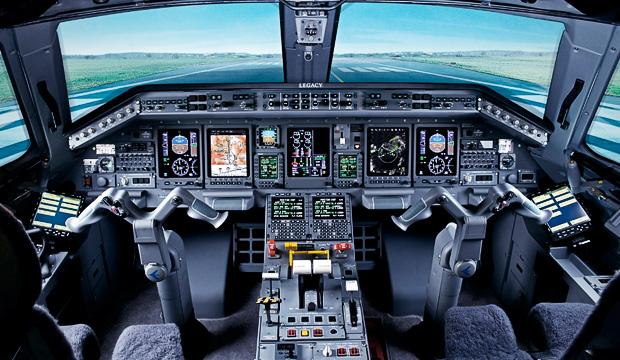
\includegraphics[height=4cm]{media/cockpit.jpg}
    \end{columns}
}

\frame{
    \frametitle{Why is HCI very important?}
    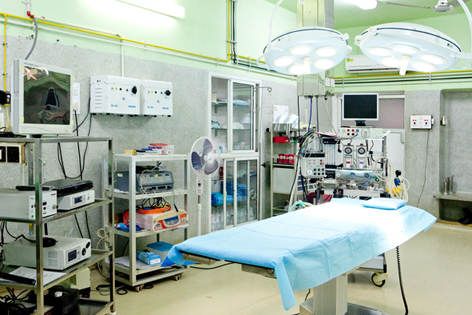
\includegraphics[height=6cm]{media/ot_1.jpg}
}

\frame{
    \frametitle{Why is HCI very important?}
    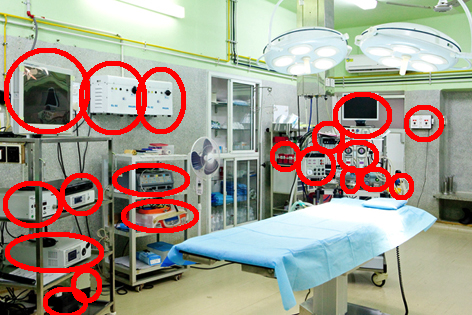
\includegraphics[height=6cm]{media/ot_2.jpg}
}

\frame{
    \frametitle{Aspects of HCI}
    \begin{description}[Hardware interface]
        \item [Software interface] (components, layout, colours, etc.)
        \item [Hardware interface] (buttons, screen size) 
        \item [Responsiveness] (is action too slow?)
        \item [Feedback] (do we need progress bars?)
        \item [Adaptiveness] (ease of learning)
        \item [Ergonomics] (physical ease of use)
    \end{description}
    ... And many more.
}

\frame{
    \frametitle{HCI is subjective}
    \begin{itemize}
        \item Interface designing is very \alert{subjective}
        \item Generally, no `right' or `wrong' answers
        \item \alert{Justification} is important
        \item However, there are guidelines...
    \end{itemize}
}

\frame{
    \frametitle{Getting stuff wrong: icons}
    \centering
    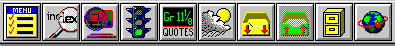
\includegraphics[height=1cm]{media/bad_buttons.png}
}

\frame{
    \frametitle{Getting stuff wrong: user control}
    \centering
    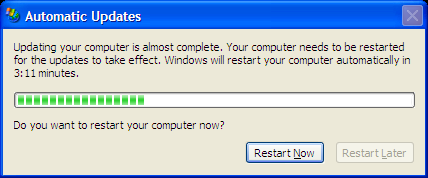
\includegraphics[height=4cm]{media/restart.png}
}

\frame{
    \frametitle{Getting stuff wrong: Windows in general}
    \centering
    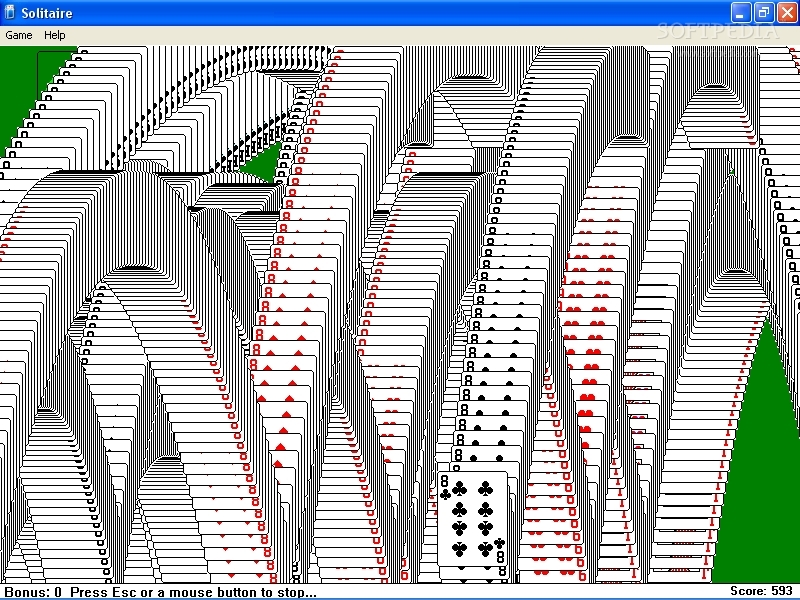
\includegraphics[height=7cm]{media/solitaire.jpg}
}

\frame{
    \frametitle{Getting stuff wrong: colours}
    \centering
    
\includegraphics[height=4cm]{media/stop.jpeg}
}

\frame{
    \frametitle{System planning}
    \begin{block}{Feature/scope creep}
        Modifying requirements or adding features during the development phase, or at any non-planning phase. 
    \end{block}
    \vskip10pt
    This can lead to overcomplicated interfaces as more features are squeezed in.    
    \vskip10pt
    \centering
    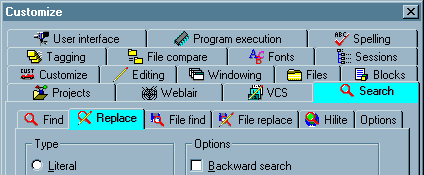
\includegraphics[height=3cm]{media/bad_tabs.png}
}

\frame{
    \frametitle{System planning}
    \begin{block}{Edge use-cases}
        Remember to consider less common situations when designing interfaces, such as cases of longer-than-usual text or weirdly-sized images.
    \end{block}
    \vskip20pt
    \centering
    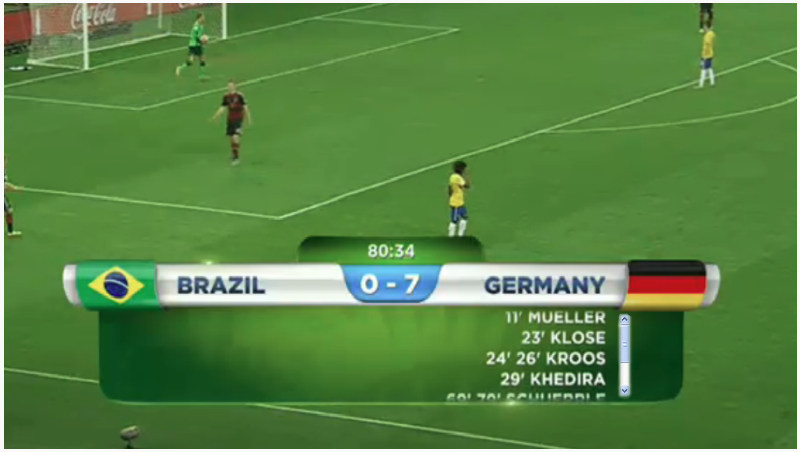
\includegraphics[height=4cm]{media/brazil_germany.jpg}
}

\frame{
    \frametitle{Human factors}
    Designers need to consider physiology of the human \alert{body}. Ask yourself:
    \begin{itemize}
        \item What inputs does the system need? (Text, image, temperature, etc.)
        \item What is the best way for a human to provide input? (Voice, typing, moving)
        \item What colours are naturally appropriate?
        \item How much contrast do I need to make this stand out? 
    \end{itemize}
    
    \vskip30pt
    We should also consider human \alert{diversity}, for example:
    \begin{itemize}
        \item Using colours visible to colourblind people.
        \item Designing inputs and outputs for able, less-able, and disabled people. 
    \end{itemize}
}

\frame{
    \frametitle{Usability}
    \alert{How user-friendly is the system?}
    \vskip10pt
    \begin{description}[Learnability]
        \item [Learnability] Easiness to learn
        \item [Efficiency] Quickness of use
        \item [Visibility] How obvious the state of the system is
        \item [Errors] Are errors descriptive and recoverable?
        \item [Satisfaction] Is it enjoyable to use?
    \end{description}
}

\frame{
    \frametitle{Human factors in usability}
    Remember that \alert{you} are not the user.

    We need to cater for many user types:
    \begin{itemize}
        \item Experts
        \item Novices
        \item Users with some knowledge of the system's domain
        \item Users with some \textit{general} techincal knowledge
        \item Users with experience with using \textit{your} system
    \end{itemize}
}

\frame{
    \frametitle{Summary}
    \begin{itemize}
        \item HCI is the study of combining humans with technological systems
        \item It is bridging psychology with technology
        \item Human factors:
            \begin{itemize}
                \item How humans can provide input and receive output from the system
                \item Human physiology is important to consider
                \item How best to design systems to work with humans
                \item Ensure systems are usable and safe to use
            \end{itemize}
        \item Usability is to do with how well users can use the system
            \begin{itemize}
                \item How \alert{effectively} users can use the system
                \item \alert{Efficiency} of the system
                \item \alert{Safety} of the system
            \end{itemize}
    \end{itemize}
}
\end{document}
